\section{Diskussion}
\label{sec:Auswertung}
\todo[inline, color=red]{Vera}
\begin{figure}[H]
	\subfigure{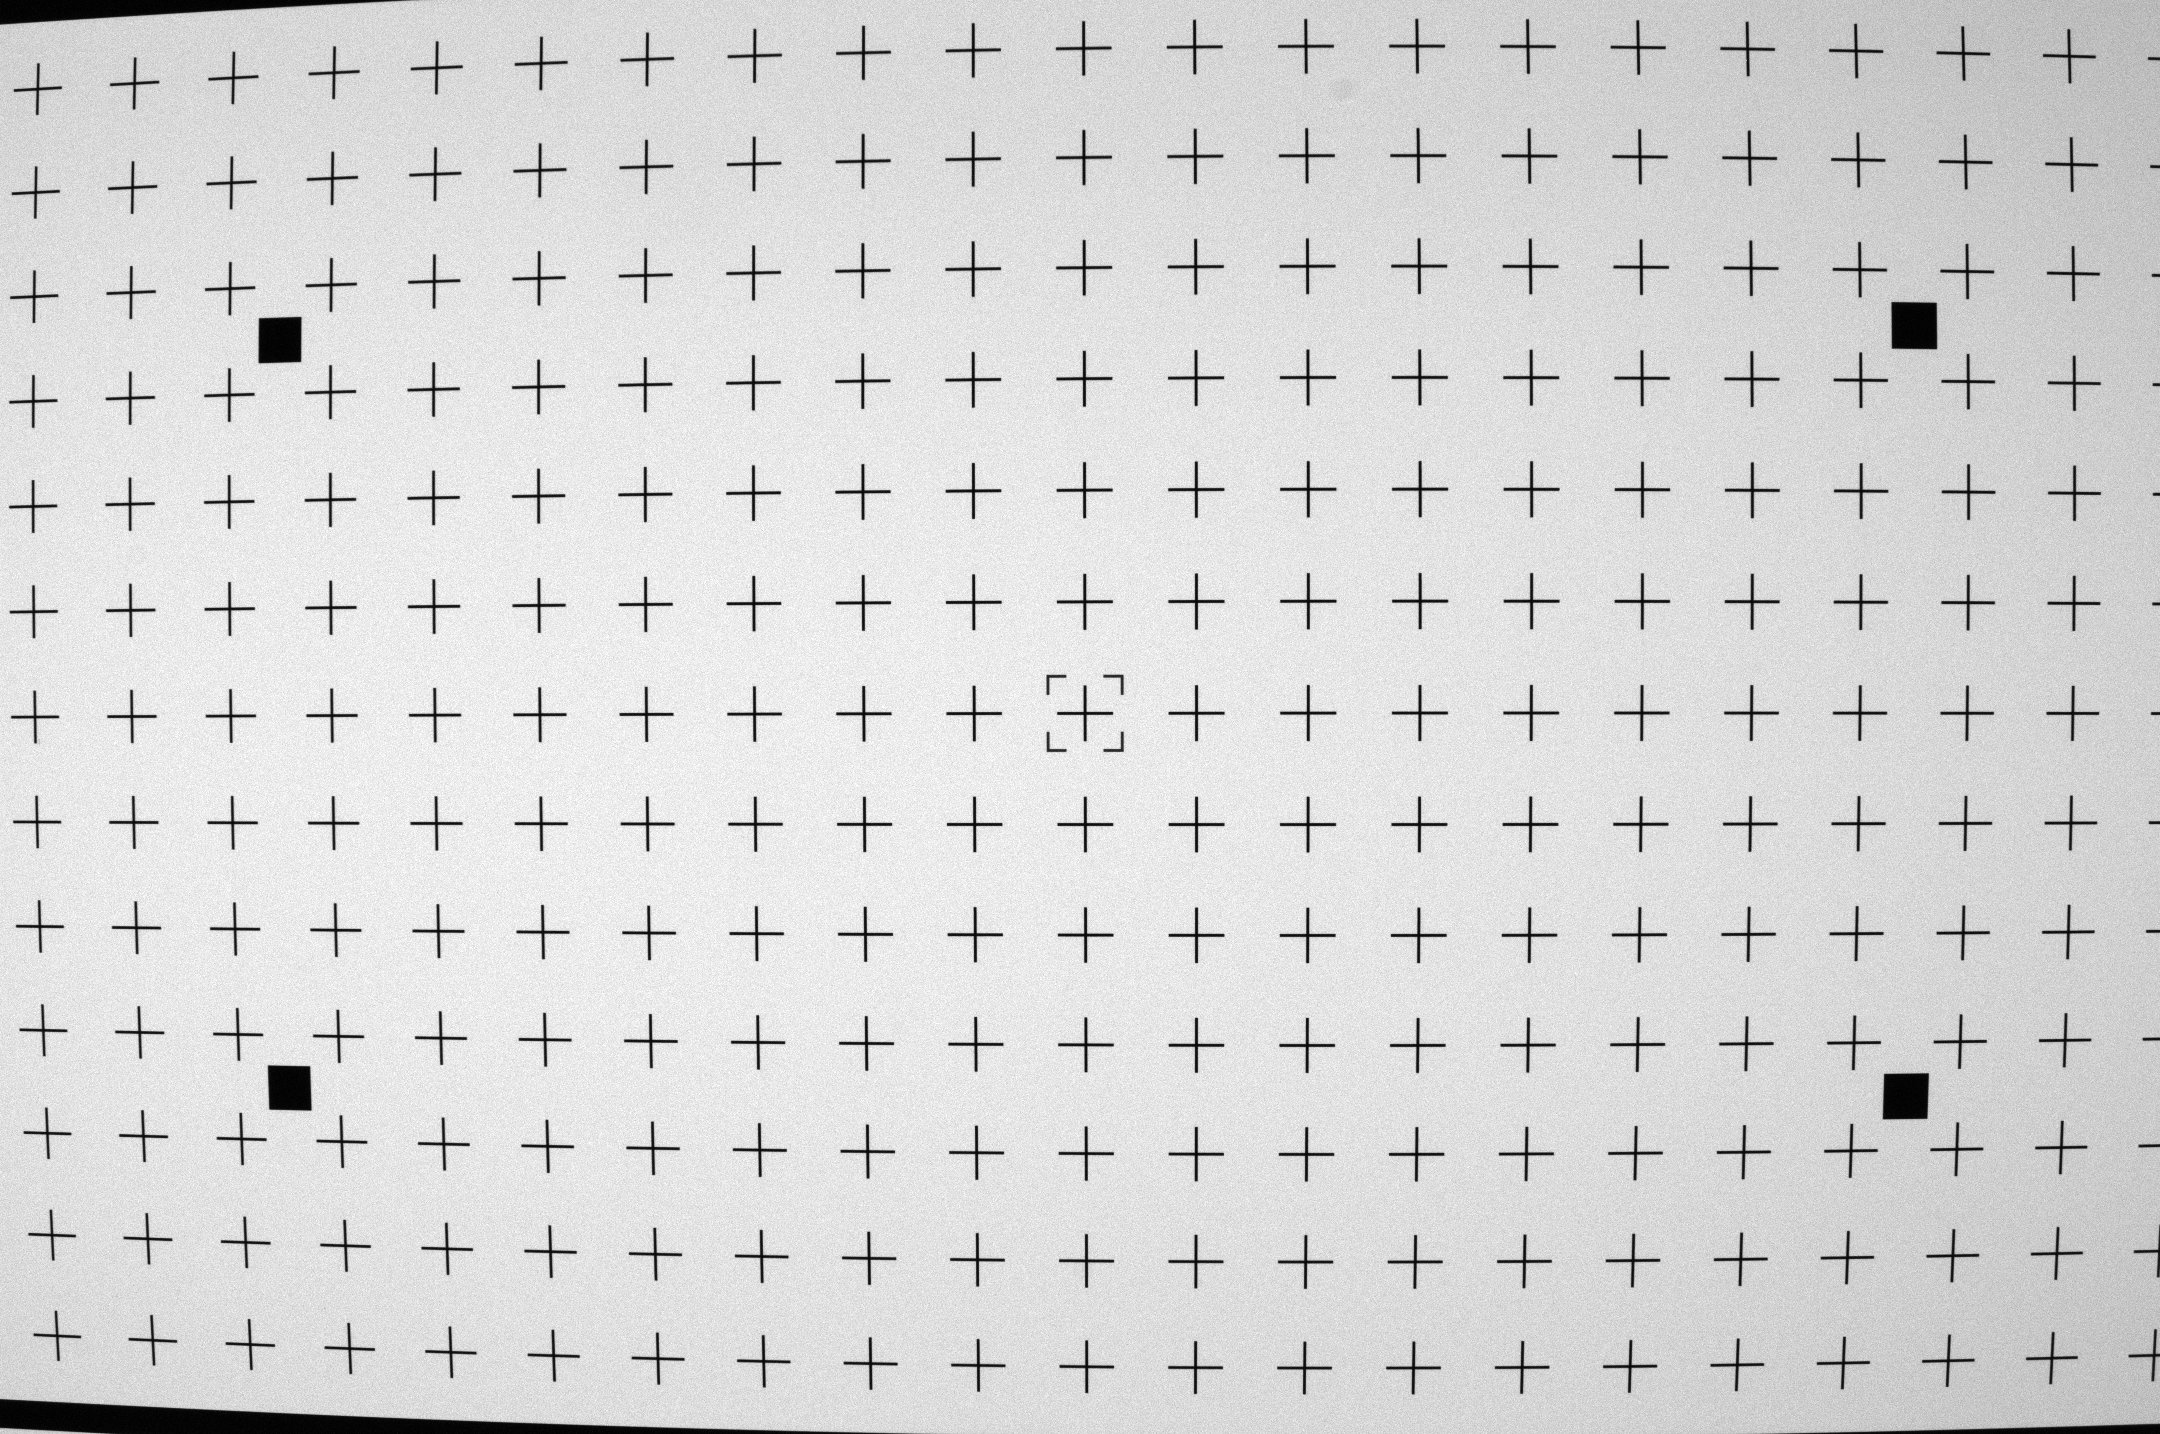
\includegraphics[width=\textwidth/2]{Images/Auswertung/Testbild1/18mm_11-1.jpg}}
	\subfigure {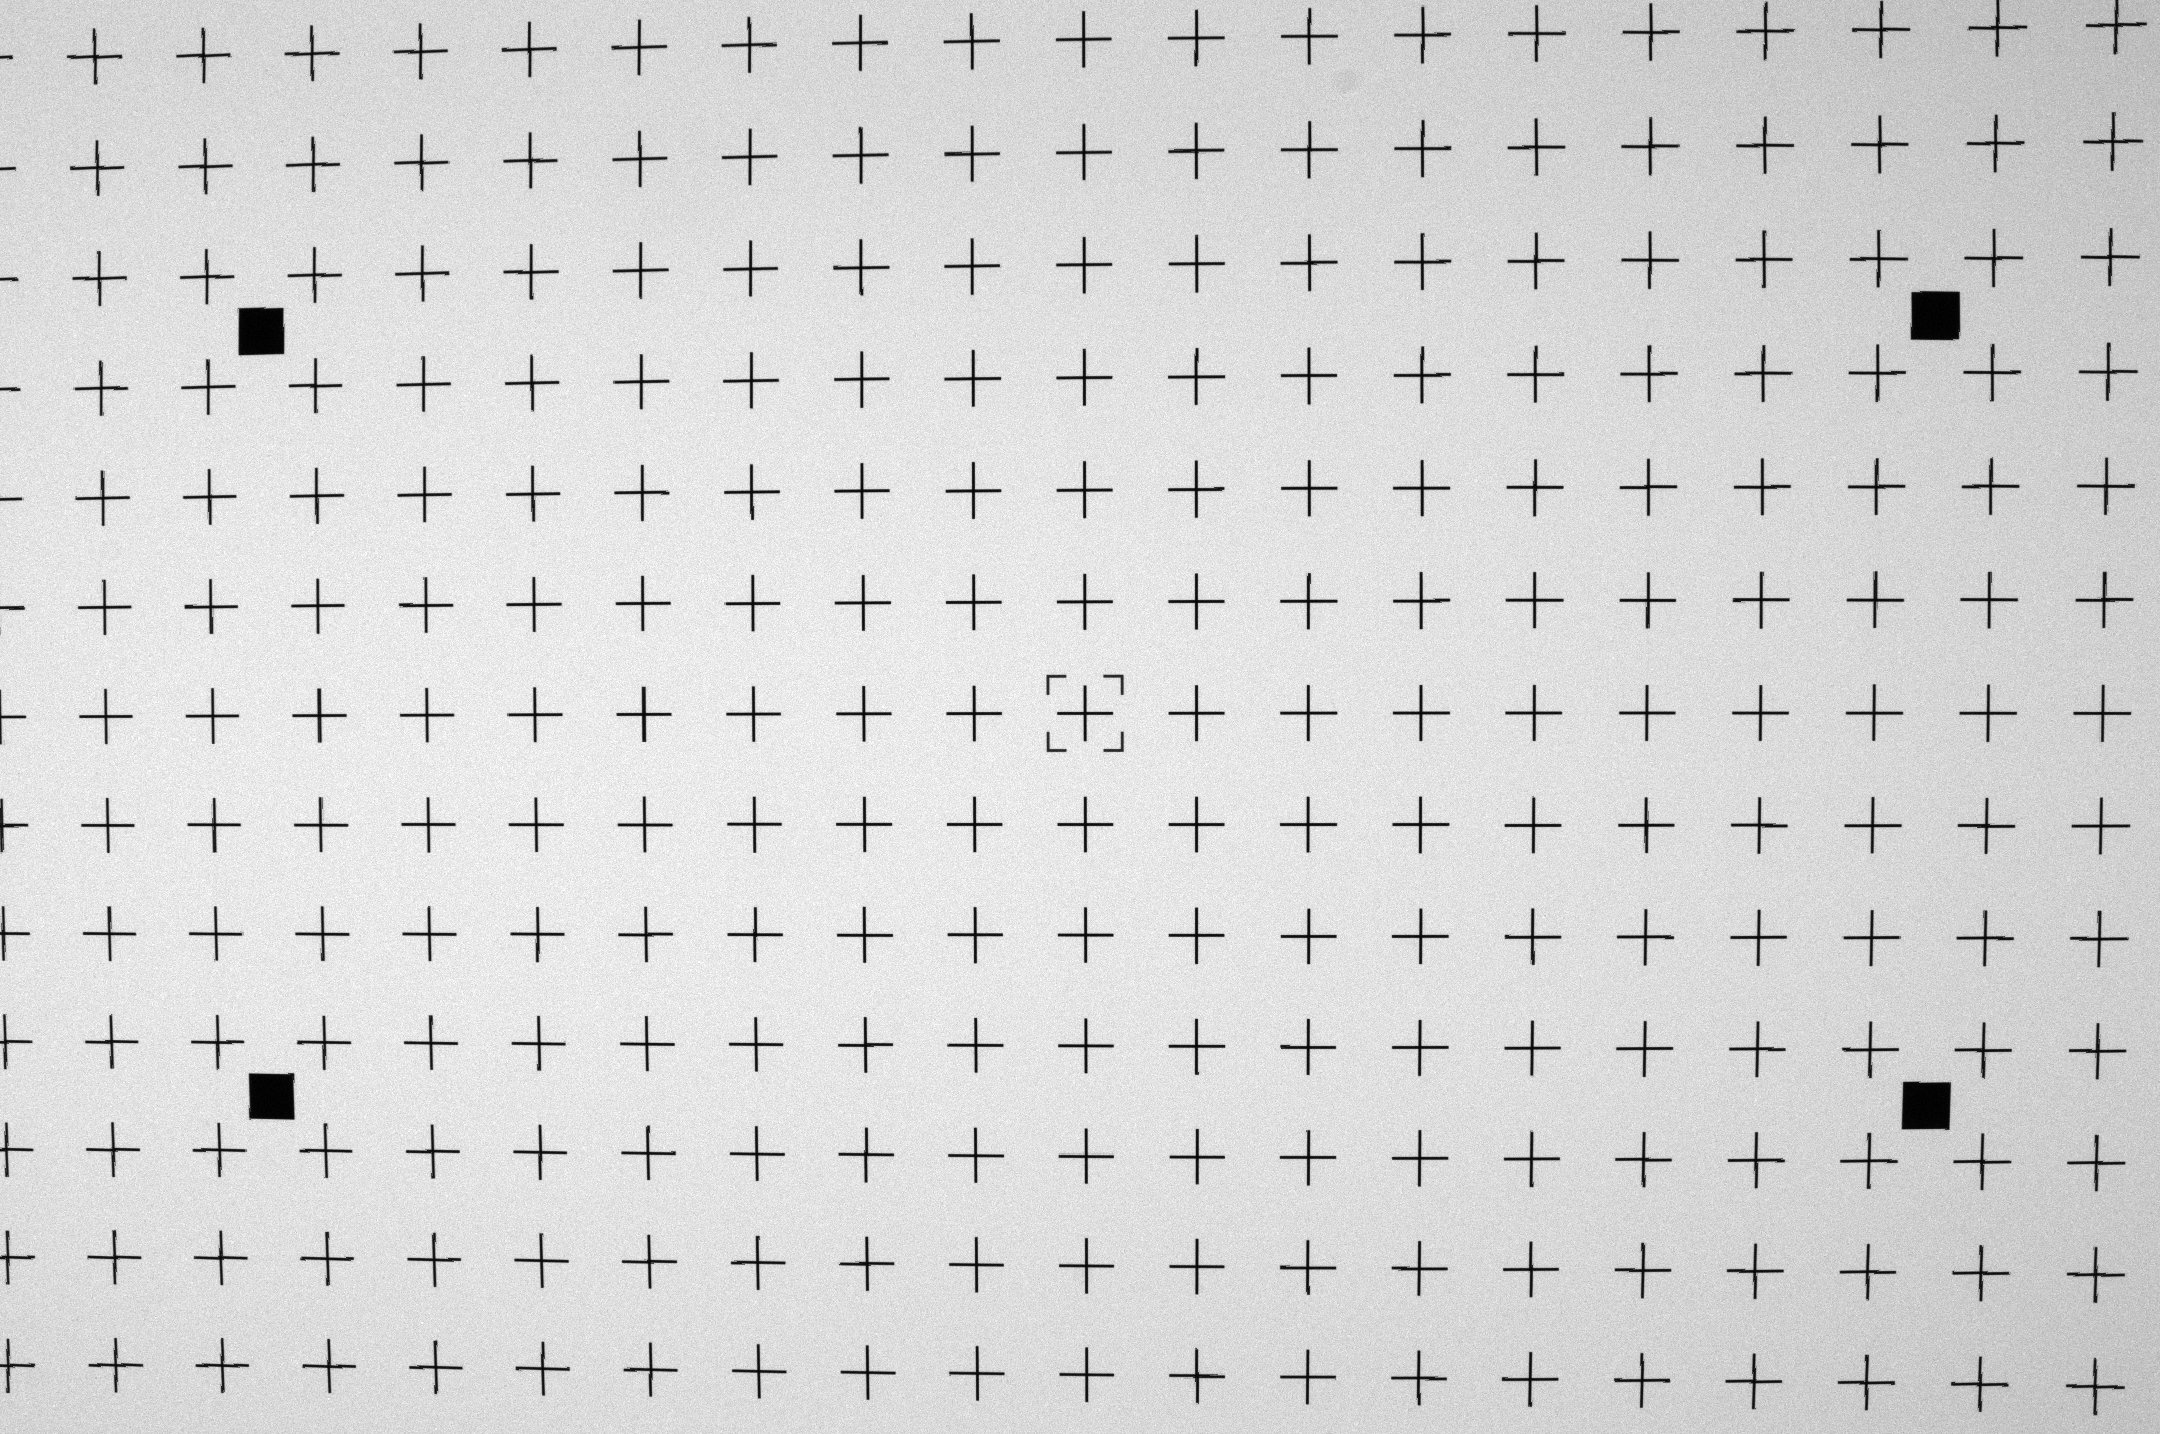
\includegraphics[width=\textwidth/2]{Images/Auswertung/Testbild1/Radial.jpg}}
	\caption{Links: Ausgangsbild. Rechts: Resultat der Radialen Entzerrung}
	\label{fig:Ergebnis}
\end{figure}

\begin{figure}[H]
	\subfigure {
\includegraphics[width=\textwidth/2]{Images/Auswertung/Testbild1/SourceImage with PointPairs_onlydiffs.jpg}}
	\subfigure{	
\includegraphics[width=\textwidth/2]{Images/Auswertung/Testbild1/Radial_onlydiffs.jpg}}
	\caption{Links: Differenzen zwischen den idealen und realen Stützpunkten. \\Rechts: Differenzen zwischen den idealen und transformierten Stützpunkten.}
	\label{fig:diffsResult}
\end{figure}



